\documentclass{beamer}
\usetheme{CambridgeUS}
\usecolortheme{seahorse}

\setcounter{tocdepth}{3}
\setcounter{secnumdepth}{3}

\newcounter{saveenumi}
\newcommand{\seti}{\setcounter{saveenumi}{\value{enumi}}}
\newcommand{\conti}{\setcounter{enumi}{\value{saveenumi}}}

\resetcounteronoverlays{saveenumi}

\usepackage{chronology}
\usepackage{caption}
\usepackage{xcolor,amsmath}
\usepackage{color}
\usepackage{graphicx}
\usepackage{tikz}
\usepackage{soul}

\makeatletter
\renewcommand*\env@matrix[1][*\c@MaxMatrixCols c]{%
  \hskip -\arraycolsep
  \let\@ifnextchar\new@ifnextchar
  \array{#1}}
\makeatother


\newcommand{\plain}{\color{black}}

\definecolor{c1}{RGB}{114,0,172}
\definecolor{c2}{RGB}{45,177,93}   
\definecolor{c3}{RGB}{251,0,29}    
\definecolor{c4}{RGB}{18,110,213}  
\definecolor{c5}{RGB}{255,160,109} 
\definecolor{c6}{RGB}{219,78,158}  

\newcommand{\growth}{\color{c1}}
\newcommand{\unitQuantity}{\color{c2}}
\newcommand{\unitInterest}{\color{c3}}
\newcommand{\unitTime}{\color{c4}}
\newcommand{\perfectly}{\color{c5}}
\newcommand{\compounded}{\color{c6}}

%                          Information for the Title Page
%
\title[Introduction to CT]{
	\Large Seminar: Computational Methods for X-ray Computed Tomography \\
	[5mm] \normalsize Session 1 \\
}
\author{Rayen Manai}



\institute[]{
    TU München
}
\date{19.04.2023}
\titlegraphic{%
	\vspace{5mm}%
	
\includegraphics[height=7mm]{media/tum_logo.pdf}%
	\hspace{10mm}%
}


%                                Beginning of the document 
%

\begin{document}
\begin{frame}
	\titlepage
\end{frame}

\begin{frame}
	\frametitle{Outline}
	\tableofcontents
\end{frame}

\section{Introduction}
\subsection{What is Tomography?}
\begin{frame}
	\frametitle{Surprise Egg}

\center	
	
\includegraphics[scale=0.5]{media/kinder_egg.jpg}
\end{frame}
\begin{frame}
\frametitle{The Fastest Way}
\center
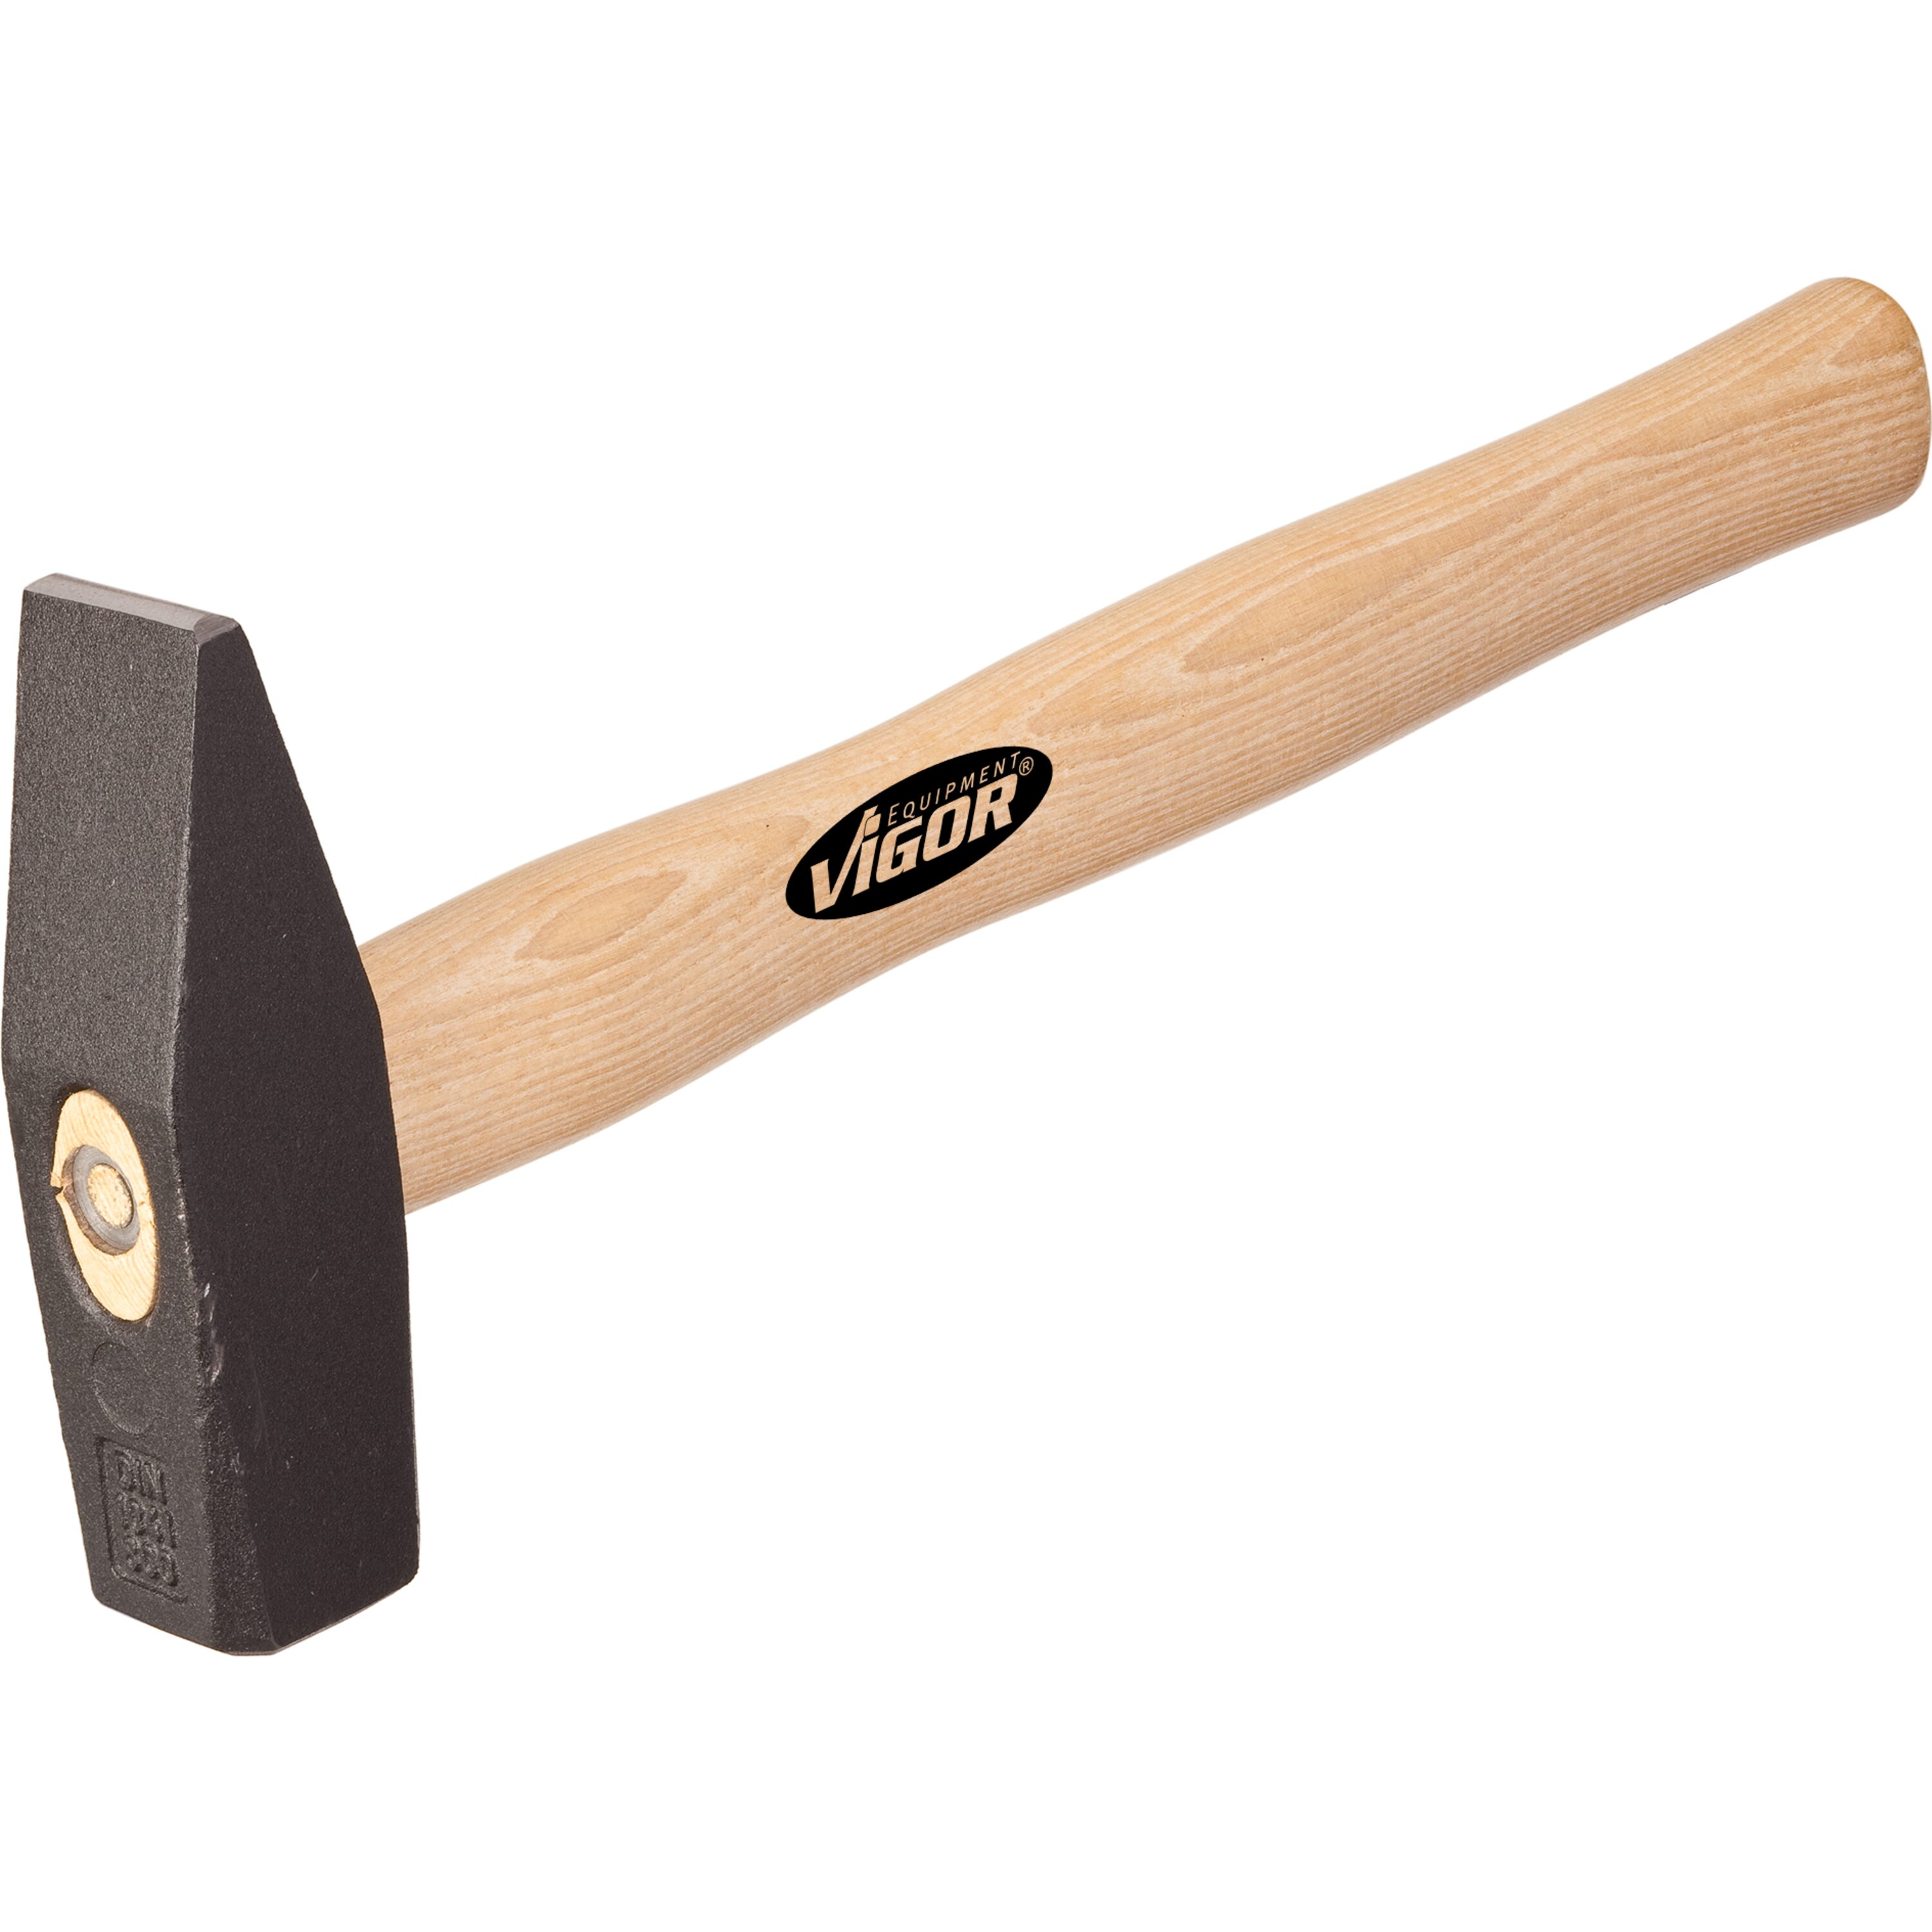
\includegraphics[scale=0.05]{media/hammer.jpg}
\end{frame}
\begin{frame}
\frametitle{The Safer Way}
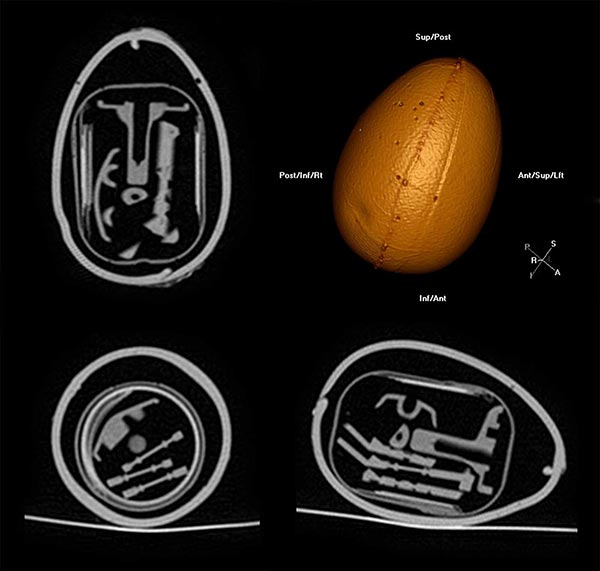
\includegraphics[scale=0.25]{media/kinder_egg_ct_slices.jpg}
\hspace{10mm}
		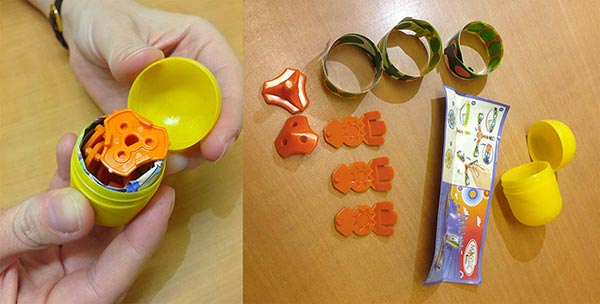
\includegraphics[scale=0.25]{media/kinder_egg_opened.jpg}
\end{frame}

\begin{frame}
	\frametitle{What is Tomography? }
	\begin{itemize}
		\item tomos(section or slice) + graphos(to describe)
		 \pause
	\item images of slices of an object without slicing it
	\item information from the outside 
		 \pause
	\item measuring the transmission of waves or
particles which more or less travel in straight lines but whose intensity is attenuated by
the material through which they travel.
	\end{itemize}

\end{frame}

\begin{frame}
	\begin{itemize}
\item tomographic reconstruction is what helps us find out what's inside things we can't look inside.
\item the process of taking projections and putting them together to form a 3D interior model
	\end{itemize}
	\end{frame}


\subsection{Important Applications of tomographic Imaging}
\begin{frame}
	\frametitle{Important Applications of tomographic Imaging}
	\begin{enumerate}
		\item Medical and biological imaging
			\begin{itemize}
				\item Clinical X-ray CT
				\item visualize damage to bones and teeth
				\item image soft tissues such as lungs
				\item electron tomography can be used to image very small objects such as viruses 
			\end{itemize}
			\seti
	\end{enumerate}
\end{frame}


\begin{frame}
	\frametitle{Important Applications of tomographic Imaging}
	\begin{enumerate}
			\conti
		\item Non destructive inspection and testing
			\begin{itemize}
				\item monitor oil and gas pipes for both their content and their integrity
				\item In museums, tomography is used to look inside artistic and cultural artifacts, archaeological finds, and fossils, without causing damage.
			\end{itemize}
	\seti
	\end{enumerate}
\end{frame}
\begin{frame}
	\frametitle{Important Applications of tomographic Imaging}
	\begin{enumerate}
			\conti
		\item Materials science
			\begin{itemize}
				\item Development of advanced materials requires understanding their properties at the micro- and nano-scale
			\end{itemize}
	\seti
	\end{enumerate}
\end{frame}
\begin{frame}
	\frametitle{Important Applications of tomographic Imaging}
	\begin{enumerate}
			\conti
		\item Security Screening
			\begin{itemize}
				\item inspect parcels and luggage, especially at airports
				\item 3D view allows objects to be seen that would otherwise be obscured by denser objects on top of them
				\item looking for bombs and weapons, tomography can be used to detect contraband
			\end{itemize}
	\end{enumerate}
\end{frame}
\subsection{CT between the past and the present}
\begin{frame}
	\frametitle{A Little History}
	\begin{chronology}[20]{1895}{2023}{60ex}[\textwidth]
	\event{1895}{X-Ray Discovery}

\end{chronology}
	\vspace{0.2cm}
	\begin{itemize}
		\item Wilhelm Conrad Röntgen produced and detected X-rays in 1895, laying the foundations in physics for X-ray scanners and tomography.
		 \pause
		\item About six weeks after his discovery, he took a picture using X-rays of his wife's hand.	
	\end{itemize}
	\center
		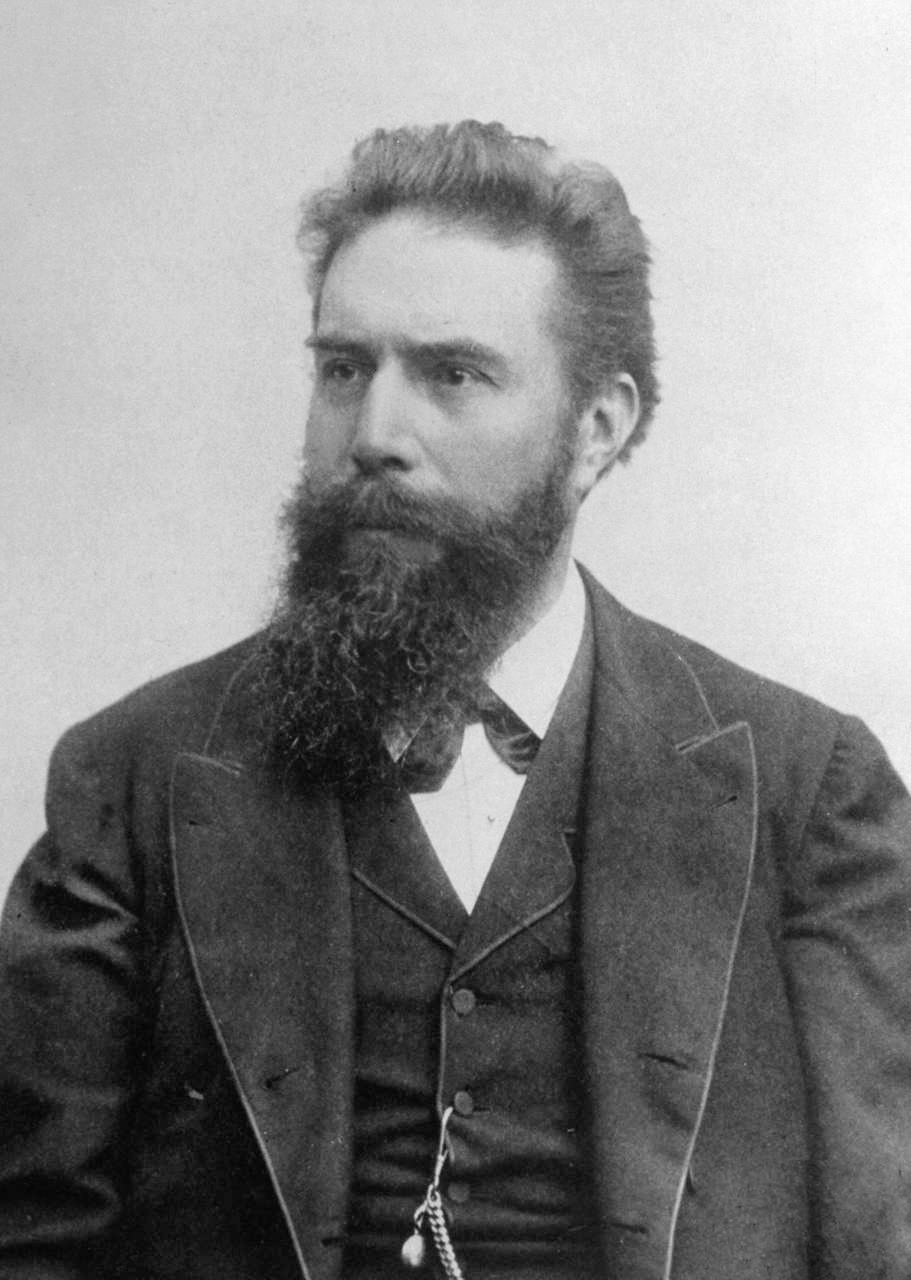
\includegraphics[scale=0.25]{media/Roentgen.jpg}
\end{frame}
\begin{frame}
	 \center
	 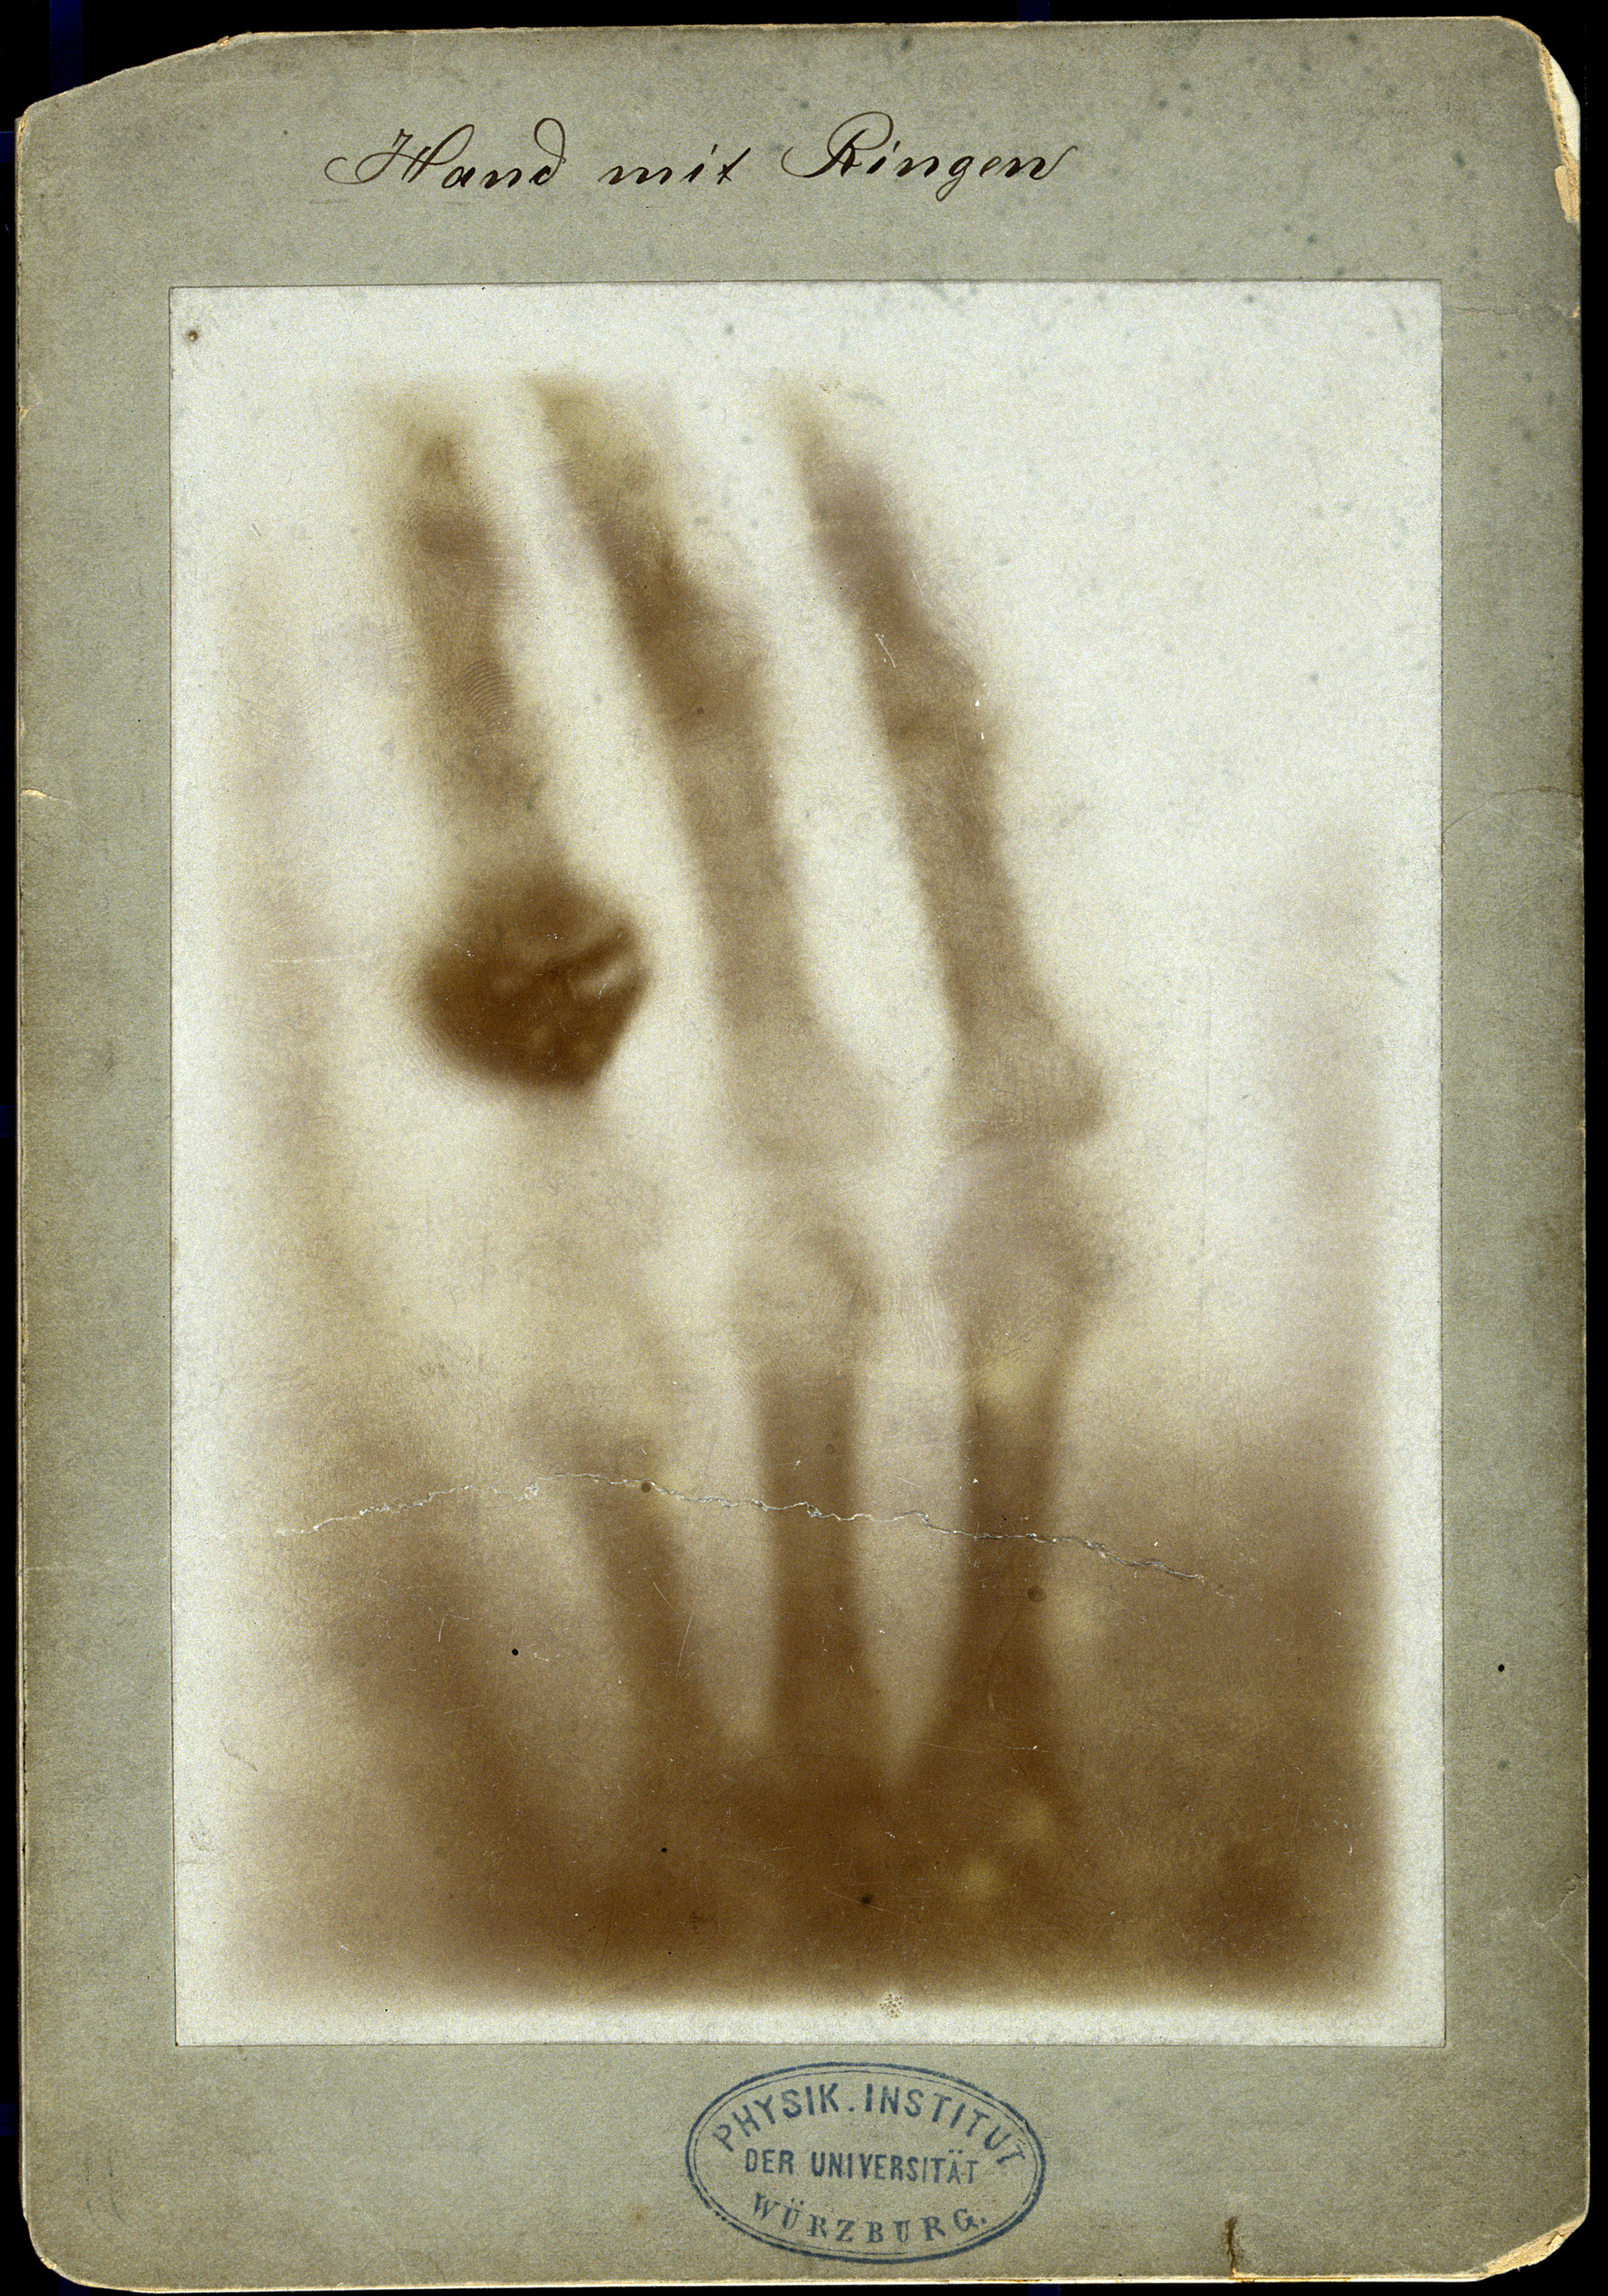
\includegraphics[scale=0.04]{media/handxray.jpg}
\end{frame}
\begin{frame}
	\begin{chronology}[20]{1895}{2023}{60ex}[\textwidth]
	\event{1917}{Johann Radon}

\end{chronology}
	\vspace{0.3cm}
	\begin{itemize}
		\item Johann Radon: published a paper 1917 about the problem of recovering a function on the plane from its line integrals.
	\end{itemize}
	\center
		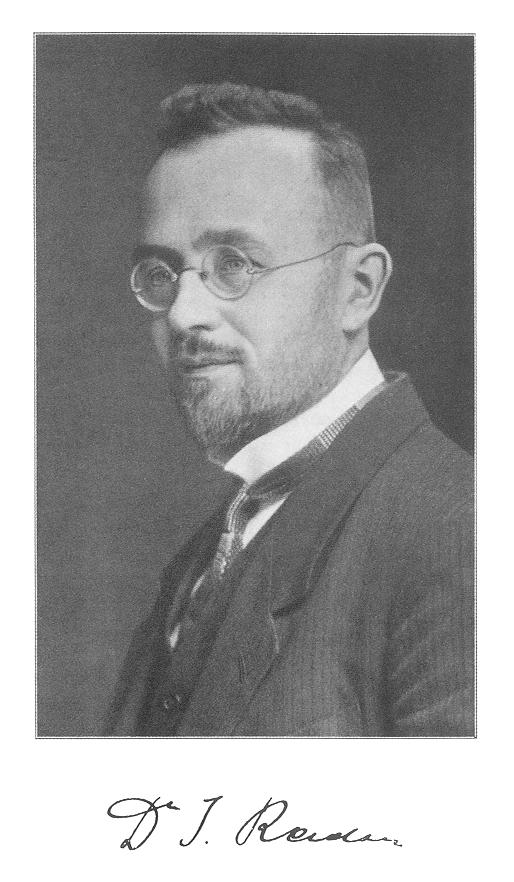
\includegraphics[scale=0.15]{media/Johann_Radon.png}
\hspace{10mm}
		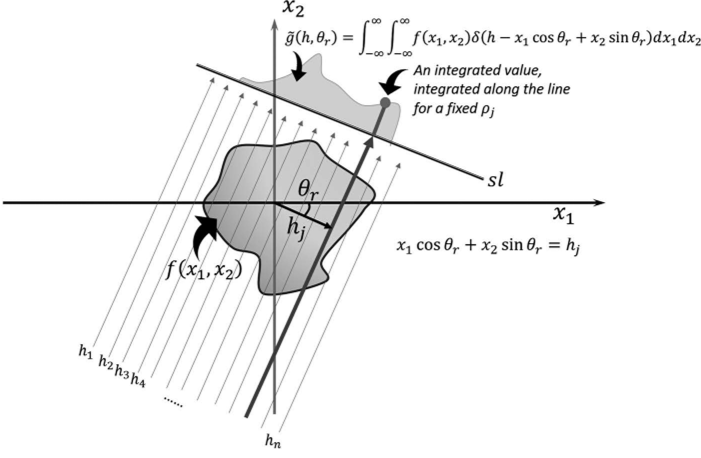
\includegraphics[scale=0.6]{media/radon_transform.png}

\end{frame}

\begin{frame}
\frametitle{A little History}
\begin{chronology}[20]{1895}{2023}{60ex}[\textwidth]
	\event[1956]{1964}{2 important papers}

\end{chronology}
	\vspace{0.5cm}
	\begin{itemize}
	\item The first proposed use: radio astronomy with Bracewell’s paper in 1956.
		 \pause
	\item The rise of tomography to the 1960s, especially with Allan Cormack’s 1963 paper.
\item Cormack's experimental measurements: published in 1964.
		 \pause
\item Godfrey Hounsfield experiments: applying X-ray CT to a preserved human brain, and then to animal brains from butcher shops.
	\end{itemize}
\end{frame}

\begin{frame}[t]
	\frametitle{A little History}
\begin{chronology}[20]{1895}{2023}{60ex}[\textwidth]
	\event[1971]{1972}{First application}
\end{chronology}
	\begin{itemize}
			\vspace{1cm}
		\item The system was first tested on a patient in 1971, and a patent was granted in 1972
	\end{itemize}
\end{frame}
\begin{frame}\frametitle{A little History}
\begin{chronology}[20]{1895}{2023}{60ex}[\textwidth]
	\event{1979}{Nobel Prize}
\end{chronology}
	\vspace{0.5cm}
	\begin{itemize}
		\item Hounsfield and Cormack jointly won the Nobel Prize in Physiology or Medicine in 1979 for the invention of X-ray CT
	\end{itemize}
		\center
		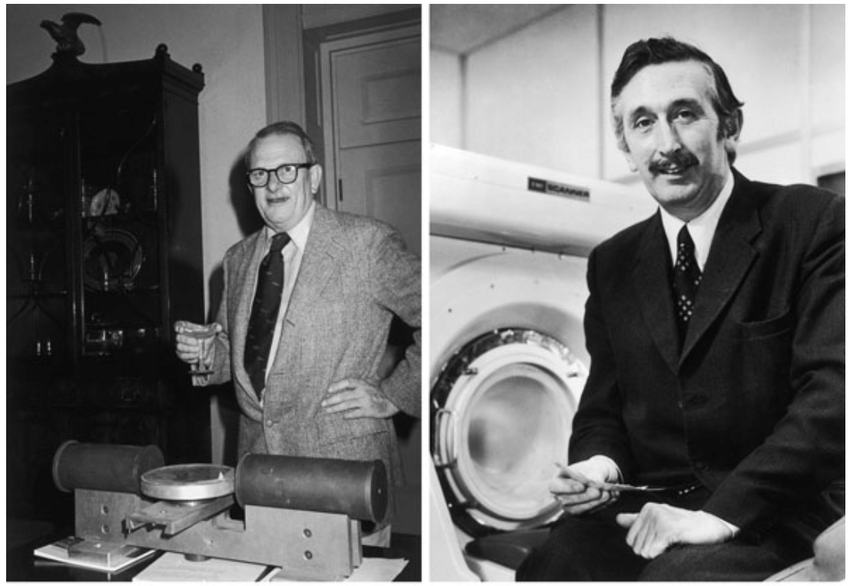
\includegraphics[scale=0.15]{media/Cormack+Hounsfield.png}
\end{frame}
\begin{frame}
	\frametitle{Tomography today}
	
	\begin{itemize}
		\item Initial applications of X-ray tomography were: diagnostic imaging and medicine 
		\item large manufacturers, such as GE Healthcare, Siemens, Philips, Toshiba, and Hitachi who produce medical CT machines
		 \pause
\item[i)] Cone-beam CT
\item modern medical CT machines use a helical-scan cone beam
\item the patient is translated on a table 
\item the X-ray source and the detector array rotate about a horizontal axis.
	\end{itemize}
\end{frame}
\begin{frame}
	\begin{itemize}	
		\item Dental cone-beam CT: widely used in dental hospitals, 
		\item for extensive surgical procedures
		\item circular-scan cone-beam geometry
	\end{itemize}
	\center
		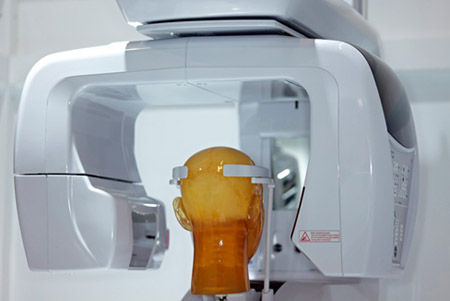
\includegraphics[scale=0.3]{media/dental_cone_beam.jpg}
\end{frame}
\begin{frame}
	\begin{itemize}
		\item[ii)] Positron Emission Tomogrpahy
		\item PET scans use a radioactive tracer to show how an organ is functioning in real time.
		\item The radioisotopes are selectively absorbed, allowing imaging of metabolism rather than anatomy.
		 \pause
\item can measure vital functions: blood flow, oxygen use, blood sugar (glucose) metabolism ...
\item can be combined with CT or MRI to image both metabolism and anatomy.
	\end{itemize}
	\center 
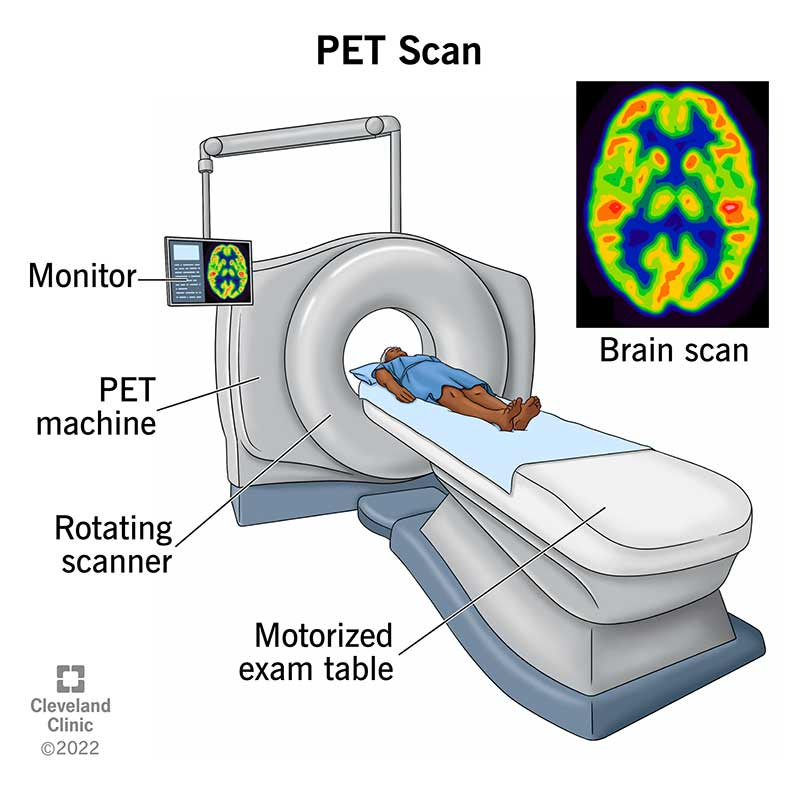
\includegraphics[scale=0.15]{media/pet-scan.jpg}
\end{frame}

\begin{frame}
	\begin{itemize}	
		\item[iii)] Transmission Electron Microscope
		\item used extensively in biology and medicine (in a technique called cryo-EM), in which the sample is frozen.
		\item Because electrons are charged particles, the beam can be directed using magnetic and electric fields
		 \pause
\item The sample must be relatively thin for the electrons to penetrate, and for that reason projections can only be collected by tilting
by around 70° either way. 
		\item a parallel-beam limited-angle problem.
		 \pause
 \item used, e.g., to image virus particles. (The Electron Microscopy Data Bank reported that 200 out of the 250 protein structures
registered in 2020 were found using electron tomography)
	\end{itemize}
	\end{frame}
	 \begin{frame}
		 \begin{itemize}
			\item widely used in materials science to understand smaller structures than is possible using X-ray tomography. 
			\item uses a scanning transmission electron microscope (STEM), where a pencil beam of high-energy electrons is focused into a narrow beam which is raster scanned
			\item or an ordinary TEM, in which the full object is illuminated by a parallel beam
	\end{itemize}
		 \center 
		 \pause
\begin{figure}
  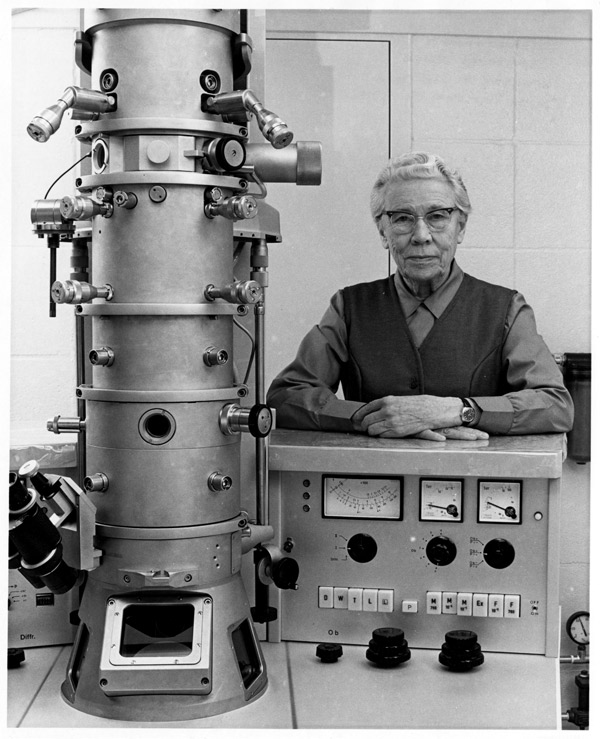
\includegraphics[scale=0.15]{media/Esau_at_TEM.jpg}
  \caption{Katherine Esau next to her TEM}
\end{figure}


\end{frame}

\begin{frame}
	\frametitle{Tomography today}
	\begin{itemize}	
		\item [iv)] Synchrotron X-Ray source
		\item X-ray tomography at a higher resolution than possible on a laboratory system
		\item a high-intensity beam that is highly collimated and close to monochromatic. 
		 \pause
		\item located at large national or multinational facilities such as the Diamond Light Source at Harwell in the UK or the European Synchrotron Radiation Facility (ESRF) in Grenoble, France. 
		\item high cost of the facilities.
	\end{itemize}
\end{frame}


\subsection{Aim and contents of this book}
\begin{frame}
	\frametitle{Aim and contents of the book}
	\begin{itemize}
	 \item chapters 2, 3: necessary mathematical theory and concepts
		 \pause
	 \item chapter 4: the physics of X-ray tomography
		 \pause
	 \item chapter 5: the Radon transform that takes the image to the data.
		 \pause
	 \item chapter 6: The most common family of analytical inversion methods, FBP
		 \pause
	 \item chapter 7: Limited-data problems: singular values and functions of the Radon transform.
	\end{itemize}
\end{frame}
\begin{frame}
\begin{itemize}
\item chapter 8: employs tools from microlocal analysis to look carefully at what can and cannot be stably retrieved from such restricted data.
		 \pause
\item chapter 9: The process of going from a continuum problem to a discrete one
		 \pause
\item chapter 10: This marks a transition from problems in functional analysis to a focus on numerical linear algebra and optimization.
		 \pause
\item chapter 11: the numerical linear algebra approach to image reconstruction in tomography
		 \pause
\item chapter 12: inverse problems and regularization, a trade-off between fitting the data and imposing prior assumptions about the image.
		 \pause
\item chapter 13: modern practical optimization methods that can be applied to tomographic imaging
\end{itemize}
\end{frame}

%--------------------------------------------------------------------------------------
\section{Analysis Background}
\subsection{Setting the stage: Definitions}
\begin{frame}
	\frametitle{Linear Operators}
	\begin{itemize}
		\item operator = a function that takes a function and gives another function.
		 \pause
		\item Notation: for an operator $K$, we denote by $K[f]$ the function $f$ it is taken
			to and by $K[f](x)$ its value at a real number $x$
		 \pause
		\item The range is the set of all functions $K[f]$ for some valid $f$, and it is often a smaller set than the co-domain.
		 \pause
		\item most of the problems in tomography will be formulated as an operator that takes an image to some data.

	\end{itemize}
\end{frame}

\begin{frame}
	\frametitle{example 1: Integration}
	For a function $f$ : $[-\pi, \pi] \rightarrow [-\pi,\pi]$, we can regard the operation: 
	$$ K[f](y) \; \; = \; \; \int_{-\pi}^{y} f(x) \,dx$$
	as an operator whose domain and co-domain are integrable functions on the interval $[-\pi, \pi] $ 
	\newline 
	Integrating a function makes it a little smoother, so in this example the range is a smaller set than the co-domain.
\end{frame}
\begin{frame}
	\frametitle{Linearity of an operator}
	We say an operator is linear if it has both the superposition property 
	$$  K[f1 + f2] \; = \; K[f1] + K[f2]$$ 
	for any two functions f1 and f2 in the domain and the scaling property 
	$$ K[\alpha f] \; = \; \alpha K[f]$$
	for any function f in the domain and any scalar $\alpha$ .

\end{frame}

\begin{frame}
	\frametitle{How to combine two functions ?}
	\center
	Suppose I give you two different functions and I ask you to think of all the ways you might combine the two functions to get a new function.
\end{frame}
\begin{frame}
\frametitle{How to combine two functions ?}
\center
	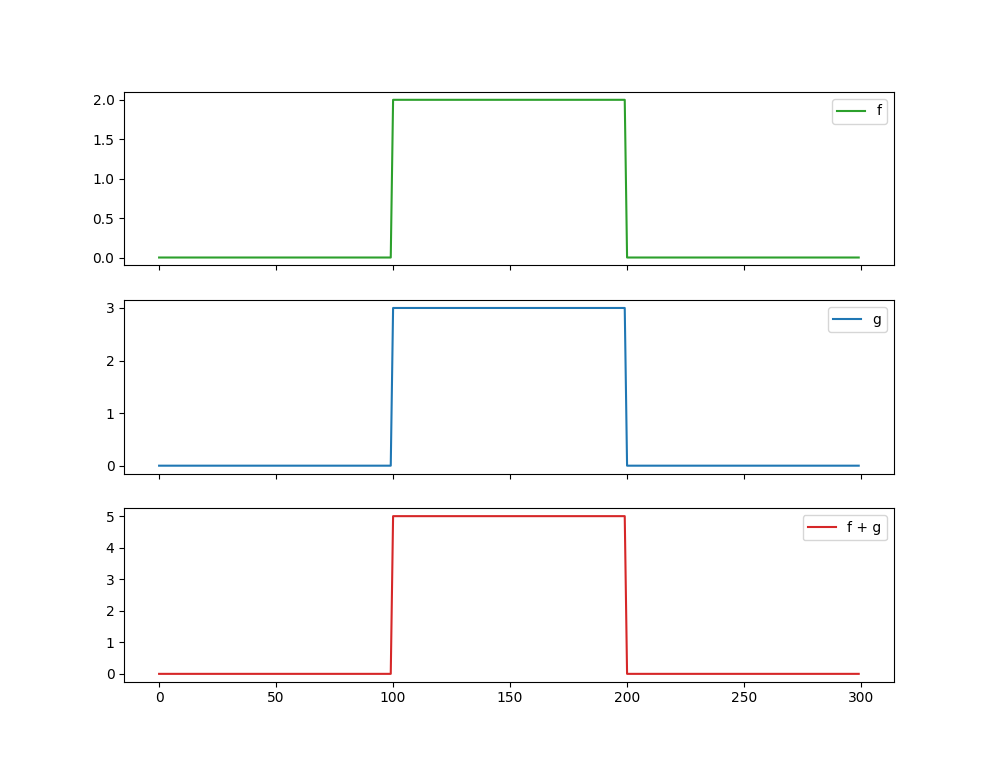
\includegraphics[scale=0.4]{media/added.png}

\end{frame}

\begin{frame}
	\frametitle{How to combine two functions ?}
\center
	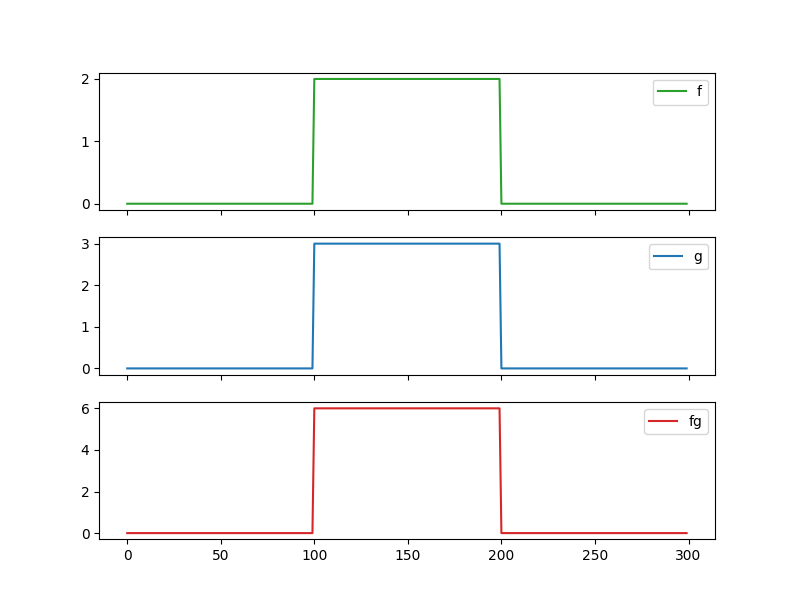
\includegraphics[scale=0.5]{media/multiplied.png}

\end{frame}
\begin{frame}
	\frametitle{How to combine two functions ?}
\center
	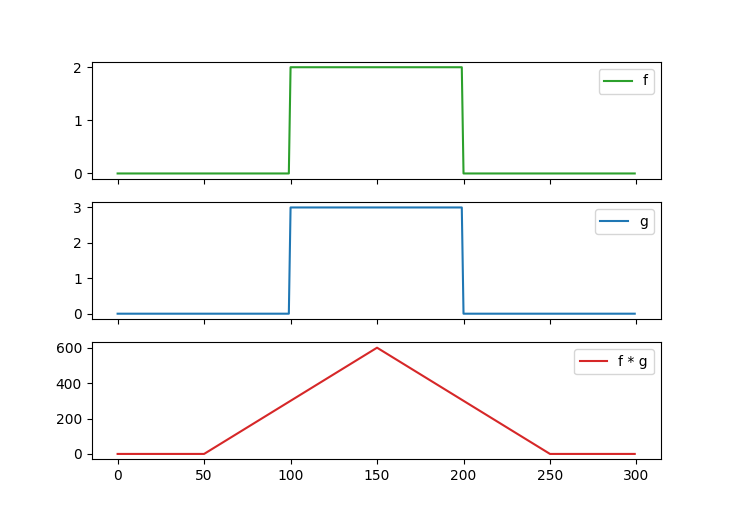
\includegraphics[scale=0.5]{media/convolved.png}

\end{frame}
\begin{frame}
	\frametitle{example 2: Convolution operator for periodic functions}
	We consider again $2\pi$-periodic functions on the interval $[-\pi, \pi]$, and we define the convolution operator as: 
	$$ g(x)  =  K[f](x)  = \int_{-\pi}^{\pi} h(y - x )f(y) \, dy $$  or $$ g  =  h * f$$
		 \pause
	\begin{itemize}
		\item $h$ defines the system (periodic) 
		\item $y-x$ wraps around when it goes outside the interval $[-\pi, \pi]$
		\item we refer to convolution of periodic functions as circular convolution
	\end{itemize}
\end{frame}
\begin{frame}
	\frametitle{General form of convolution}
	%% source : https://betterexplained.com/articles/intuitive-convolution/
	$$\plain ( 
	\growth f
\perfectly *
\unitTime g
	\plain )
	\plain (
	\unitInterest t
	\plain )
\plain =
	\unitQuantity \int_{-\infty}^{\infty} \growth f(\tau)
	\unitTime g(\unitInterest t \compounded -\tau \unitTime) \unitQuantity d\tau 
$$
\perfectly To convolve
\growth       a kernel
\plain        with an 
\unitTime input signal :
\
\compounded flip the signal
\unitInterest move to the desired time 
\unitQuantity and accumulate every interaction  
\growth with the kernel

\end{frame}
\begin{frame}
	\frametitle{Visualization}
\end{frame}
\begin{frame}
	\frametitle{example 3: Integration as Convolution}
We can formulate the integration operator in Example 1 as a convolution by choosing: 
	$$ h(x) = \begin{cases}
	1, \; \; x \in [-\pi, 0]  , \\
        0,  \; \; x \in ]0,\pi]  ,
\end{cases} $$
so that 
	$$ h * f(x) = \int_{-\pi}^{x} f(y) \, dy $$ 
\end{frame}
\subsection{Inverse Problems and Regularization}
\begin{frame}
	\center 
	We will now discuss the inverse process of computing or reconstructing the function f from the data g, which we refer to
as an inverse problem.
\end{frame}
\begin{frame}
	\frametitle{What is an inverse problem?}
\begin{center}
\begin{tikzpicture}
	\node (pic1) at (0,0) {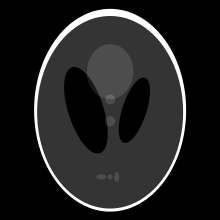
\includegraphics[width=0.15\textwidth]{media/SheppLogan_Phantom.png}};
\node (pic2) at (7,0) {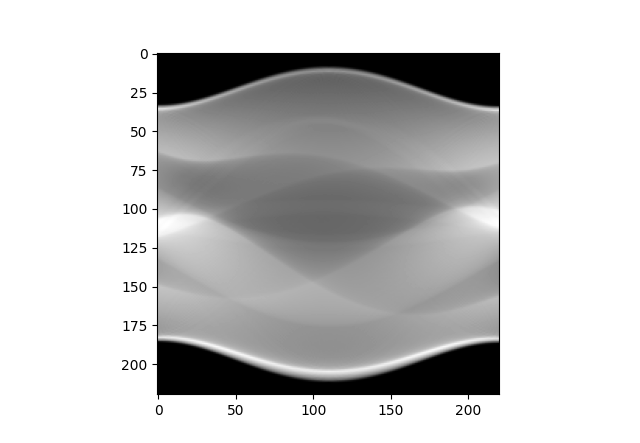
\includegraphics[width=0.25\textwidth]{media/sinogram.png}};
\draw[->,thick] (pic1.east) -- ++(2.2,0) |- (pic2.west) node[pos=0.5,above] {Direct Problem};
\end{tikzpicture}
\end{center}
\center
	Direct problem: given object $f$ determime data $y$
\end{frame}
\begin{frame}
	\frametitle{What is an inverse problem?}
\begin{center}
\begin{tikzpicture}
	\node (pic1) at (0,0) {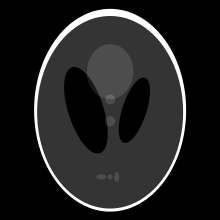
\includegraphics[width=0.15\textwidth]{media/SheppLogan_Phantom.png}};
\node (pic2) at (7,0) {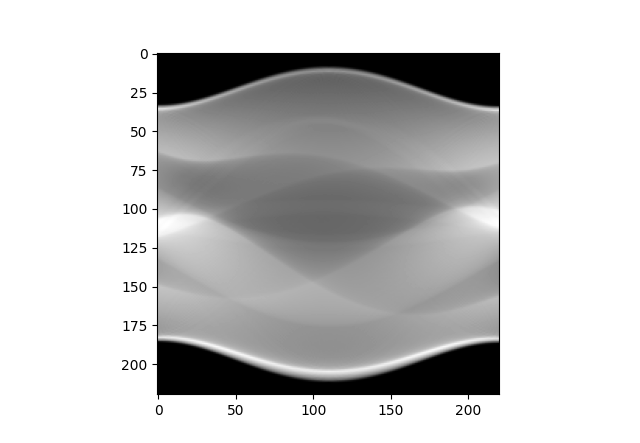
\includegraphics[width=0.25\textwidth]{media/sinogram.png}};
\draw[->,thick] (pic2.west) -- ++(-2.2,0) |- (pic1.east) node[pos=0.5,below] {Inverse Problem};
\end{tikzpicture}

	Inverse problem: given noisy data $ \hat{y}$, recover object $f$
	\newline 
		 \pause
	Solving the inverse problems means reconstructing the object from the measured
data

\end{center}
	
\end{frame}
\begin{frame}
	\frametitle{What is an inverse problem?}
	\begin{itemize}
		\item estimate a quantity f that is not directly observable using indirect measurements g and the forward model, the operator K. 
		 \pause
		\item The forward problem is a model for how the observations arise
		\item the inverse problem is a model for how, from a set of observations, we compute the causal factors that produced them.
		 \pause
\item an inverse problem typically takes a “forward problem,” such
as “given the properties of the interior of the object, how much of an X-ray beam penetrates the object,” 
			\item attempts to invert it: deducing interior information from these exterior measurements 
	\end{itemize}
\end{frame}

\begin{frame}
	\begin{itemize}
		\item Typically the forward problem is a natural process, i.e., “solved” by physics. 
		 \pause
		\item As humans, we choose an inverse problem to solve, which is perhaps why such problems are often so difficult
		 \pause
		\item The Three Important Questions of Inverse Problems
			\begin{enumerate}
				\item What do you need to find?
		 \pause
				\item What can you measure?
		 \pause
				\item What do you already know?
			\end{enumerate}
	\end{itemize}
\end{frame}
\begin{frame}
	\frametitle{Sensitivity to noise}
	\begin{itemize}
		\item CT images can be affected by noise, which can result in reduced image quality and potentially lead to diagnostic errors.
		 \pause
		\item The noise can arise from various sources, such as electronic noise in the CT detector, scattered radiation, or patient motion during the  scan.
		 \pause
		\item $\rightarrow $artifacts in the reconstructed image, such as streaks or blurring
		\item necessity to minimize the noise in CT to improve image quality and diagnostic accuracy.
		 \pause
		\item Filtering: a technique that involves modifying pixel values in an image to reduce noise while preserving image details.
	\end{itemize}
\end{frame}
\begin{frame}
	\frametitle{Applying a Gaussian Filter to a noisy signal}
	\center
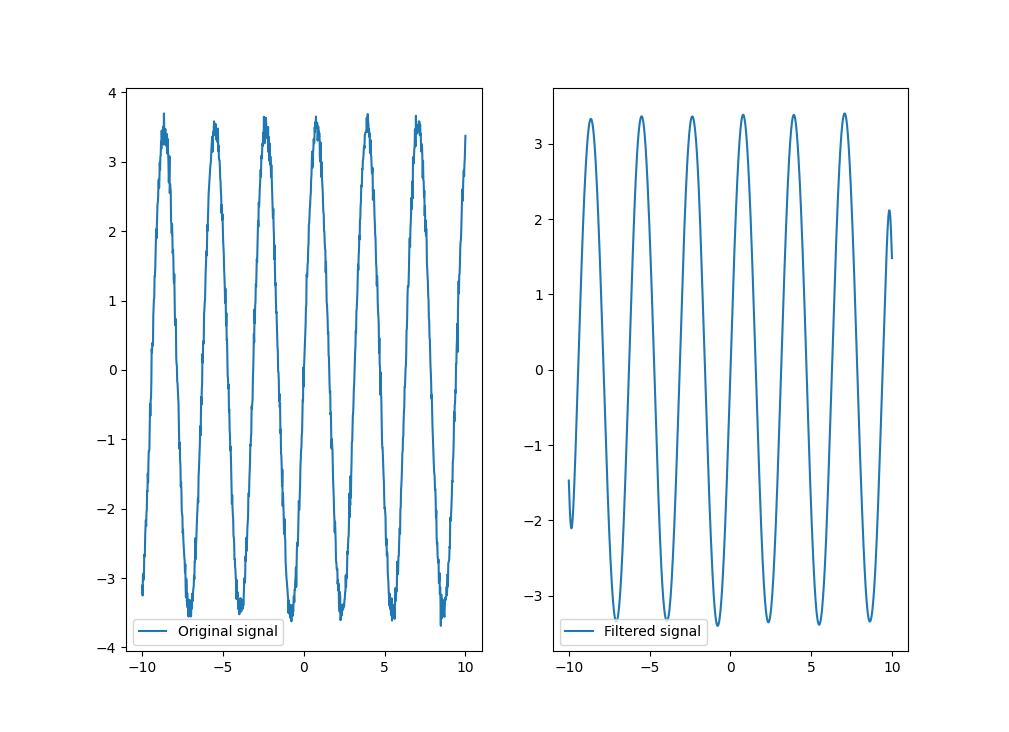
\includegraphics[scale= 0.4]{media/noise_separated.png}
\end{frame}
\begin{frame}
	\frametitle{Applying a Gaussian Filter to a noisy signal}
	\center
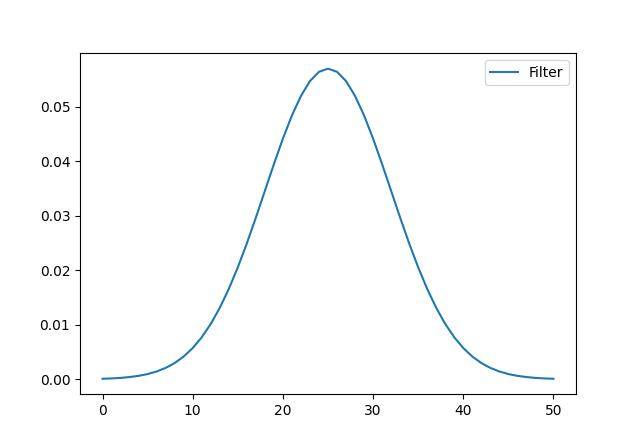
\includegraphics[scale= 0.5]{media/gaussian.png}
\end{frame}
\begin{frame}
	\frametitle{Applying a Gaussian Filter to a noisy signal}
	\center
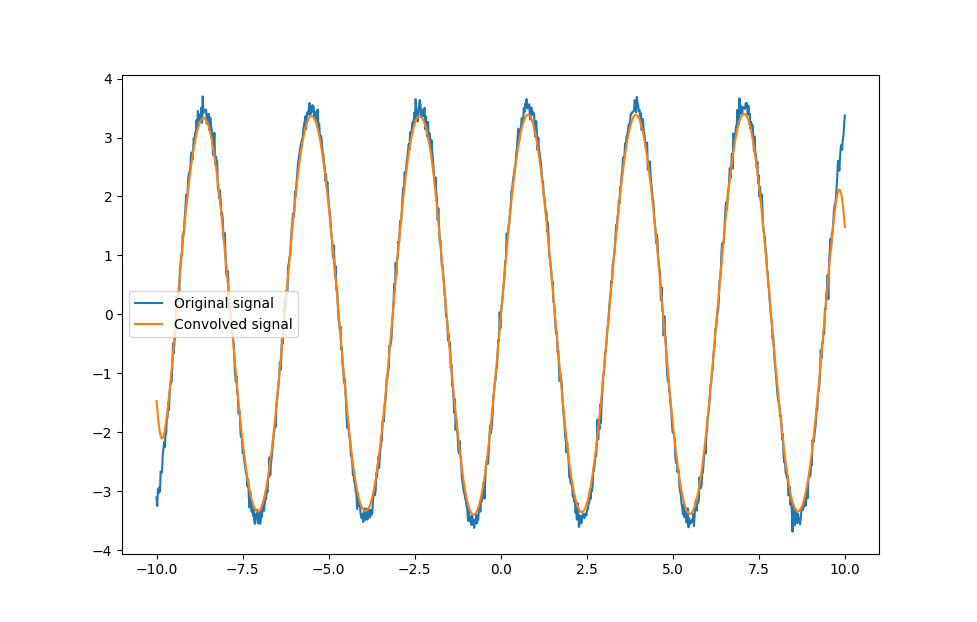
\includegraphics[scale= 0.4]{media/noise_mixed.png}
\end{frame}

\begin{frame}
	\center
Inverse problems can be quite difficult to solve.
This is because many inverse problems are ill posed, according to the following definition.
\end{frame}

\begin{frame}
\frametitle{Well-Posed and Ill-Posed Problems}
\begin{columns}
\begin{column}{0.4\textwidth}
\centering
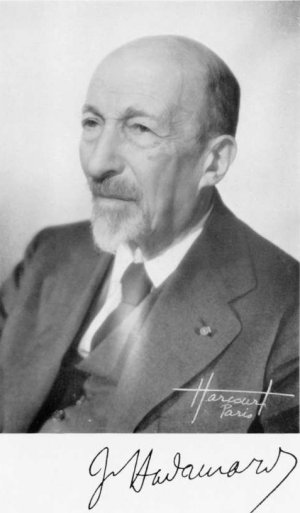
\includegraphics[scale= 0.5]{media/Hadamard.jpg}
\end{column}
\begin{column}{0.6\textwidth}
Hadamard’s criteria for a well-posed problem are : 
\begin{itemize}
		 \pause
	\item a solution exists
		 \pause
	\item the solution is unique, and
		 \pause
	\item the solution depends stably on the data
\end{itemize}
		 \pause
If a problem violates any of these criteria, we say that it is ill posed.
\end{column}
\end{columns}
\end{frame}

\begin{frame}
	\begin{itemize}
          \item	The solution exists if g is in the range, the set of all $K[f]$ for all valid $f$
		 \pause
	  \item Often a solution might not exist due to errors such that the measured data g has a component
outside the range
		 \pause
\item A unique solution means that $K$ has an inverse $K^{-1}$ so that $K^{-1}[K[f]] = f $
	\end{itemize}
\end{frame}
\begin{frame}
	\frametitle{Stability}
	\begin{itemize}
		\item The solution is \colorbox{green!30}{stable} if \colorbox{green!30}{any perturbation of the data} g produces a \colorbox{green!30}{bounded perturbation of the solution f}
		 \pause
		\item \colorbox{red!30}{instability: } a small \colorbox{red!30}{perturbation in the data} can make an arbitrarily \colorbox{red!30}{large change in the solution f}
	\end{itemize}
\end{frame}
\begin{frame}
\center
Solution?
\end{frame}
\begin{frame}
	\frametitle{Stabilization by regularization}
	\center The important principle is that you can’t
beat the analysis!
\newline
As you measure more data and try to get a more accurate approximation to the solution, you approach the ill-posed continuum problem
with its inherent instability
\end{frame}

\begin{frame}
	\frametitle{Stabilization by regularization}
	\begin{itemize}
		\item Suppose the operator $K : U \rightarrow V  $ has a bounded inverse
		\item but, the noisy data $g$ lives in a co-domain larger than the range
		\item $\rightarrow$ There is no $f$ such that $ K[f] = g$ the first Hadamard criterion is violated 
		
	\end{itemize}
		 \pause
	To overcome this, it is common to instead consider a solution that minimizes a norm of the residual $K[f] - g$ 
	$$ f_{min} = argmin_{f} || K[f] - g ||_{V}^{2} $$
\end{frame}

\begin{frame}
	\frametitle{Stabilization by regularization}
	Regularization: a class of solution methods designed to make the solution regular, stable with respect to perturbations:
		 \pause
	\begin{itemize}
		\item altering the reconstruction so the modified problem satisfies the three Hadamard criteria, generally known as Tikhonov regularization (more in the discrete setting in chapter 12)
		 \pause
		\item regularizing the solution by introducing filters in the expansion (filtering techniques in Chapters 6, 7, 10, 11 and 12)
		 \pause
		\item terminate an iterative solver before the noise starts to dominate the reconstruction (this approach is discussed in Chapter 11)
		
	\end{itemize}
\end{frame}

\subsection{The Fourier Transform}

\begin{frame}
	\frametitle{The Fourier Transform}
There are various conventions in defining the Fourier transform. Here, we define the Fourier transform for a function $f$ of one variable $x$ by
	$$ \hat{f(\omega)} = \frac{1}{\sqrt{2\pi}} \int_{-\infty}^{\infty}f(x)e^{-ix\omega} \, dx$$ 
where the Fourier-transformed function $f$ is a function of the angular frequency $\omega$. 
\newline 
		 \pause
The inverse Fourier transform of a function f is then defined as
	$$ \check{f(x)} = \frac{1}{\sqrt{2\pi}} \int_{-\infty}^{\infty}f(\omega)e^{ix\omega} \, d\omega$$ 
\end{frame}
\begin{frame}
	\frametitle{The Fourier Transform}
	\begin{itemize}
		\item The Fourier transform gives the frequency components of a function
		\item The Fourier transform of a real function is complex, encoding both the magnitude and the phase of the frequency components
		\item We say “in frequency space” or “in Fourier space” to mean considering the Fourier transform of functions with respect to the frequency variable.
	\end{itemize}
\end{frame}
\begin{frame}
	\frametitle{Examples}
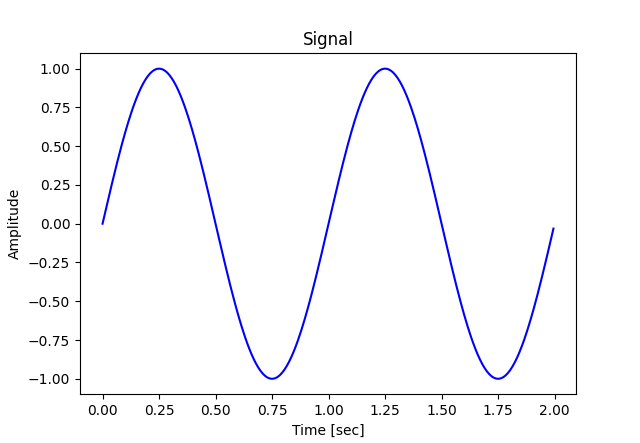
\includegraphics[scale = 0.35]{media/signal1.png}
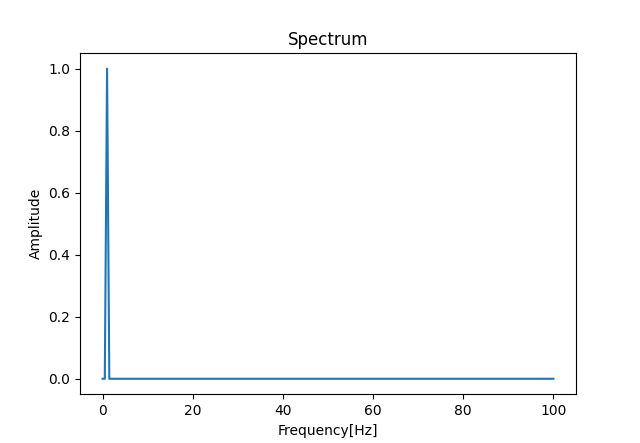
\includegraphics[scale = 0.35]{media/fourier1.png}	
\end{frame}

\begin{frame}
	\frametitle{Examples}
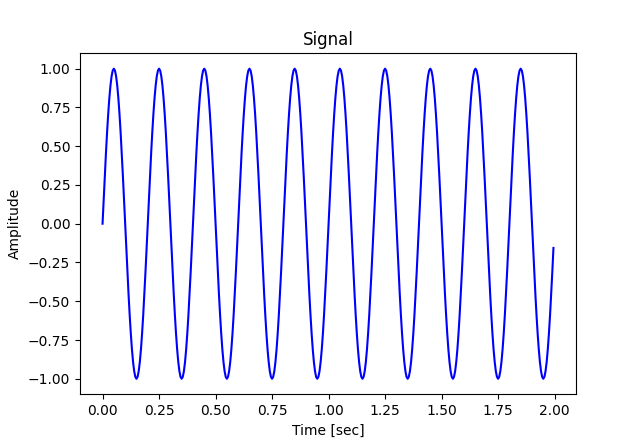
\includegraphics[scale = 0.35]{media/signal2.png}
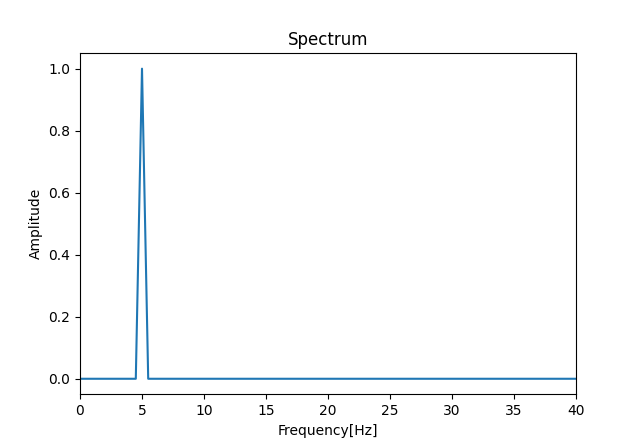
\includegraphics[scale = 0.35]{media/fourier2.png}	
\end{frame}
\begin{frame}
	\frametitle{Examples}
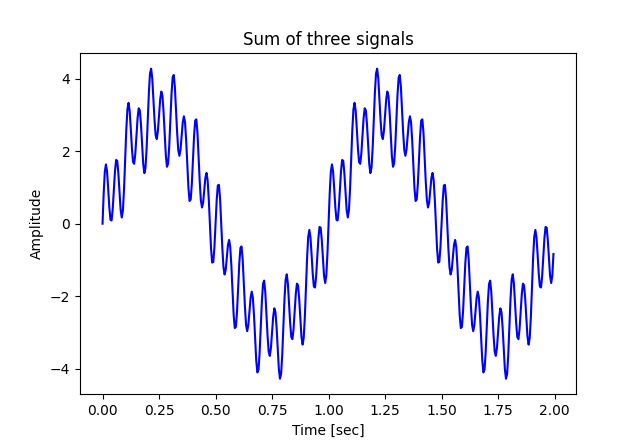
\includegraphics[scale = 0.35]{media/signal3.png}
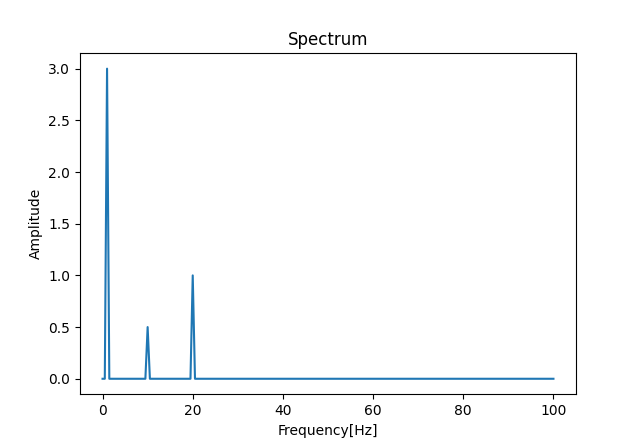
\includegraphics[scale = 0.35]{media/fourier3.png}	
\end{frame}
\begin{frame}
	\frametitle{The 2D Fourier Transform}
	Let $f$ be a function of $x = (x_1,x_2)$. The the 2D Fourier Transform is a function of the angular frequency vector $\omega = (\omega_{1},\omega_{2})$ given by 
	$$ \hat{f(\omega)} = \frac{1}{2\pi}\int_{-\infty}^{\infty} \int_{-\infty}^{\infty}f(x)e^{-ix\omega} \, dx_{1}dx_{2}$$ 
	where $ x\omega = x_1\omega_{1} + x_2 \omega_{2}$
\newline 
		 \pause
The 2D inverse Fourier Transform is
	$$ \check{f(x)} = \frac{1}{2\pi}\int_{-\infty}^{\infty} \int_{-\infty}^{\infty}f(\omega)e^{ix\omega} \, d\omega_{1} d\omega_{2}$$
	$\rightarrow$ The 2D Fourier transform is just the 1D Fourier transform with respect to each of the variables in turn.
\end{frame}
\begin{frame}
	\frametitle{Quiz}
	\center
Which of the following propreties hold?
	\vspace{1cm}
\begin{itemize}
		 \pause
	\item $ \alpha f_1(x) + \beta f_2(x) \xrightarrow{\text{Fourier Transform}} \alpha F_1(\omega) + \beta F_2(\omega)$
		 \pause
	\item $ f(ax)  \xrightarrow{\text{Fourier Transform}}  \frac{1}{|a|}F(\frac{\omega}{a})$
		 \pause
	\item $ f(x)h(x)  \xrightarrow{\text{Fourier Transform}}F(\omega)H(\omega)$
\end{itemize}
\end{frame}
\begin{frame}
	\frametitle{Quiz}
	\center
Which of the following propreties hold?
	\vspace{1cm}
\begin{itemize}
	\item \colorbox{green!30}{$ \alpha f_1(x) + \beta f_2(x) \xrightarrow{\text{Fourier Transform}} \alpha F_1(\omega) + \beta F_2(\omega)$: Linearity}
	\item \colorbox{green!30}{$ f(ax)  \xrightarrow{\text{Fourier Transform}}  \frac{1}{|a|}F(\frac{\omega}{a})$: Scaling}
	\item \colorbox{red!30}{$f(x)h(x)  \xrightarrow{\text{Fourier Transform}}F(\omega)H(\omega)$}
\end{itemize}
\end{frame}


\begin{frame}
	\frametitle{Convolution and Fourier Transform}
\begin{center}
\begin{tabular}{|c|c|}
\hline
\textbf{Spatial Domain} & \textbf{Frequency Domain} \\
\hline
	$g(x) = f(x)*h(x) $& $G(\omega) = F(\omega)H(\omega)$ \\
	$\downarrow$ & $\downarrow$ \\
	Convolution & Multiplication
\end{tabular}
\end{center}
\end{frame}

\begin{frame}
	\frametitle{Convolution using Fourier Transform}
\center
	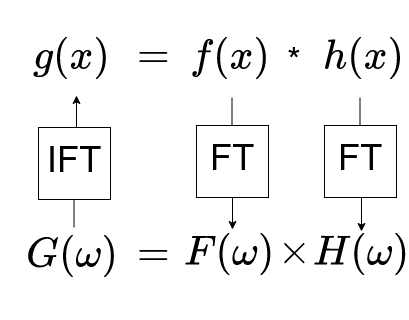
\includegraphics[scale =0.6]{media/convolution&fourier.png}
\end{frame}

%--------------------------------------------------------------------------------------
\section{Linear Algebra Background}
\subsection{System of linear equations}
\begin{frame}
\frametitle{Systems of Linear Equations}
	\begin{itemize}
	\item discretize a CT reconstruction Problem 
	\item we arrive at a system of linear equations:
	$$ Ax = b$$
		 \pause
	\item A represents a linear operator 
	\item b vector holding the measured data
	\item x the unkown solution: the reconstruction we want to compute
	\end{itemize}
\end{frame}

\begin{frame}
	\frametitle{Notation}
	column vector: $ v = \begin{pmatrix} v_1 \\ \vdots \\ v_n \end{pmatrix} \;$ , 
	row vector: $v^\top = \begin{pmatrix} x_1 & x_2 & \cdots & x_n \end{pmatrix} $
		\newline 
		 \pause
		If the matrix $A$ has dimensions $ m \times n $ (m rows and n columns), then we write it as : 
\[
A = \begin{pmatrix}
    \vert & \vert & \dots & \vert \\
    \mathbf{c_1} & \mathbf{c_2} & \dots & \mathbf{c_n} \\
    \vert & \vert & \dots & \vert
\end{pmatrix}
\quad=
\begin{pmatrix}
    \text{\textbf{r}}_1 \\
    \text{\textbf{r}}_2 \\
    \vdots \\
    \text{\textbf{r}}_m
\end{pmatrix}
\]

\end{frame}

\begin{frame}
\frametitle{example}
$$
	\begin{pmatrix} a_{11} & a_{12} \\ a_{21} & a_{22} \end{pmatrix} \;
		\begin{pmatrix} x_{1}\\ x_{2} \end{pmatrix} \;
	= \begin{pmatrix} b_{1}\\ b_{2} \end{pmatrix} \;
	$$
Two linear equations with unkowns x1 and x2 : 
$$
	a_{11}x_{1} + a_{12}x_{2} = b_{1} \; \; \; \; \; \; a_{21}x_{1} + a_{22}x_{2} = b_{2} 
$$
\end{frame}
\begin{frame}
	\frametitle{The first Problem}
	\begin{itemize}
		
\item There may not always exist an $x$ such that the equation $Ax = b$ holds.
\item	This depends on the size and the rank of the matrix $A$.
	\end{itemize}
\end{frame}


\subsection{Rank, Range and Null space}
\begin{frame}
	\frametitle{Rank}
         \begin{itemize}
\item The rank $r$ of an $ m \times n $  matrix $A$ is the number of linearly independent rows of
the matrix (it is also equal to the number of linearly independent columns), and
			 for a nonzero matrix the rank satisfies $ 1 \leq r \leq min(m,n) $
		 \pause
		 \item example : 
	 $$
		 \begin{pmatrix} 1 & 2 & 3 \\ 4 & 5 & 6 \\ 7 & 8 & 9 \end{pmatrix}  
				 \rightarrow
\begin{pmatrix} 1 & 2 & 3 \\ 0 & -3 & -6 \\ 0 & -6 & -12 \end{pmatrix}  
				 \rightarrow
\begin{pmatrix} 1 & 2 & 3 \\ 0 & -3 & -6 \\ 0 & 0 & 0 \end{pmatrix}  
				 \rightarrow $$
		 \pause
				 So this matrix has the rank $r = 2$


	 \end{itemize}
\end{frame}
\begin{frame}
	\frametitle{Range}
         \begin{itemize}
\item The range, or column space, Range($A$), of an $m \times n$ matrix $A$ is the linear
subspace spanned by the columns of the matrix:
			 $$ Range(A) \equiv \{u \in \mathbb{R}^{m} | u = \alpha_1 c_1 + \alpha_2 c_2 + \hdots + \alpha_n c_n , arbitrary \alpha_j \} $$
		 \pause
		 \item example : 
		 $$
			 \begin{pmatrix} 1 & 1 & 1 \\ 1 & 2 & 4 \\ 2 & 3 & 5 \end{pmatrix} \; 
				 \rightarrow
			 \begin{pmatrix} 1 & 0 & 0 \\ 1 & 1 & 3 \\ 2 & 1 & 3 \end{pmatrix} \; 
		         \rightarrow
		         \begin{pmatrix} 1 & 0 & 0 \\ 1 & 1 & 0 \\ 2 & 1 & 0 \end{pmatrix} \; $$
		 \pause
				 So this Matrix has Rank = 2 and $ Range (A) = \alpha_1 \begin{pmatrix} 1\\ 1 \\ 2 \end{pmatrix} \; +   \alpha_2 \begin{pmatrix} 0\\ 1 \\ 1 \end{pmatrix} \; $
	 \end{itemize}
\end{frame}

\begin{frame}
	\frametitle{Null Space (Kernel)}
         \begin{itemize}
		 \item The null space (or kernel), Null($A$), is the linear subspace of all vectors mapped to zero:
			 $$ Null(A) \equiv \{v \in \mathbb{R}^{n} | Av = 0 \} $$
		 \pause
		 \item example : 
			 $$
			 \begin{pmatrix} 1 & 1 & 1 \\ 1 & 2 & 4 \\ 2 & 3 & 5 \end{pmatrix} \; 
				 \rightarrow
			 \begin{pmatrix} 1 & 1 & 1 \\ 0 & 1 & 3 \\ 0 & 1 & 3 \end{pmatrix} \; 
		         \rightarrow
		         \begin{pmatrix} 1 & 1 & 1 \\ 0 & 1 & 3 \\ 0 & 0 & 0 \end{pmatrix} \; $$
		 \pause
				 So this Matrix has Rank = 2 and $ Null(A) = \alpha_1 \begin{pmatrix} 2\\ -3 \\ 1 \end{pmatrix} \; $

	 \end{itemize}
\end{frame}
\begin{frame}
	\begin{itemize}		
		\item The dimensions of the range and null space are $r$ and $n - r$, respectively.
		\item In the last example :
			$ n = 2 $ , $ r = 1$ and $ n - r = 1$ is the dimension of the Null space.
	\end{itemize}
\end{frame}
\begin{frame}
	\frametitle{Linear Systems}
Consider two linear sytems with the the same matrix $A$: 
	$$ \begin{pmatrix} 1 & 1 & 1 \\ 1 & 2 & 4 \\ 2 & 3 & 5 \end{pmatrix}x = \begin{pmatrix} 2\\ 4 \\ 6 \end{pmatrix} \; 
		and \begin{pmatrix} 1 & 1 & 1 \\ 1 & 2 & 4 \\ 2 & 3 & 5 \end{pmatrix}x = \begin{pmatrix} 4\\ 5 \\ 7 \end{pmatrix} \;  $$
	\begin{itemize}
		 \pause
		\item The first system, has infinitely many solutions; any vector of the form $\begin{pmatrix} 0\\ 2 \\ 0 \end{pmatrix} \; +\alpha \begin{pmatrix} 2\\ -3 \\ 1 \end{pmatrix} \; $ satisfies this equation because the last, arbitrary, component is in the null space of $A$.
		 \pause
			\item The second system has no solution because the right-hand side does not belong to the range of $A$
		
	\end{itemize}		
\end{frame}
\begin{frame}
	\frametitle{Back to CT}
	\center 
Since the data $b$ always comes from the forward projection of an image $x$, the system $Ax= b$ will always have a solution. 
\newline
\center
		 \pause
Is that true?
\end{frame}

\begin{frame}
	\frametitle{Back to CT}
         \begin{itemize}
		 \item The right-hand side that we encounter when computing a tomographic reconstruction from measured data is contaminated with noise
		 \pause
		 \item The key issue: whether the system is consistent 
		 \item whether we can find a vector $x$ that satisfies the equation 
		 \item whether the right-hand side $b$ lies in the range Range($A$)
	 \end{itemize}
\end{frame}
\subsection{Linear Least Squares Problem}

\begin{frame}
	\frametitle{Linear Least Squares Problem}
	\begin{itemize}
		\item formulation that seeks to handle inconsistency of a linear problem
		\item define a meaningful “solution” to an inconsistent system
		 \pause
		\item Idea : find an $x$ such that $ Ax$ approximates the right-hand side $b$ in some optimal way, here by minimizing the 2-norm of the residual vector $b -Ax$
	\end{itemize}
\end{frame}
\begin{frame}
	\frametitle{Formally:}
	Assume that the right-hand side has the form 
	$$ b = A\overline{x} + e$$
	\begin{itemize}
		\item $\overline{x}$ is the exact, ground truth solution
		\item $e$ is a random vector
		
	\end{itemize}
		 \pause
Then the optimal estimate of $x$ is obtained by solving the least-squares problem :
	$$x_{LS} = argmin_{x} \; \frac{1}{2} ||b - Ax||_{2}^{2} $$
\end{frame}
\begin{frame}
	\frametitle{Recipe: Compute a least-squares solution}
	Let $A$ be an $m \times n$ Matrix and $b$ a vector in $ \mathbb{R}^{n}$ 
	\begin{enumerate}
		\item[1] Compute the Matrix $A^{T}A$ and the vector $A^{T}b$ 
		 \pause
		\item[2] Form the augmented matrix for the matrix equation $A^{T}Ax = A^{T}b$ and row reduce
		 \pause
		\item[3] This equation is always consistent, and any solution $x$ is a least-squares solution.
	\end{enumerate}
\end{frame}

\begin{frame}
\frametitle{Example}
	$$\begin{pmatrix} 1 & 1 & 1 \\ 1 & 2 & 4 \\ 2 & 3 & 5 \end{pmatrix}x = \begin{pmatrix} 4\\ 5 \\ 7 \end{pmatrix}$$
		 \pause
		Ensuring the system is inconsistent: 
		$$ \begin{pmatrix}[ccc|c] 1 & 1 & 1 & 4 \\ 1 & 2 & 4 & 5 \\ 2 & 3 & 5 & 7 \end{pmatrix} 
				 \rightarrow
			 \begin{pmatrix}[ccc|c] 1 & 1 & 1 & 4 \\ 0 & 1 & 3 & 1 \\ 2 & 3 & 5 & 7 \end{pmatrix} \rightarrow$$
			$$
                         \begin{pmatrix}[ccc|c] 1 & 1 & 1 & 4 \\ 0 & 1 & 3 & 1 \\ 0 & 1 & 3 & -1 \end{pmatrix}
				 \rightarrow
                         \begin{pmatrix}[ccc|c] 1 & 1 & 1 & 4 \\ 0 & 1 & 3 & 1 \\ 0 & 0 & 0 & -2 \end{pmatrix} $$

\end{frame}
\begin{frame}
	$$ A^{T}A = \begin{pmatrix}1 & 1 & 2 \\ 1& 2 & 3 \\ 1 & 4 & 5 \end{pmatrix} 
				 \times
			 \begin{pmatrix}1 & 1 & 1 \\ 1 & 2 & 4 \\ 2 & 3 & 5 \end{pmatrix} = 
				  \begin{pmatrix}6 & 9 & 15 \\ 9 & 14 & 24 \\ 15 & 24 & 42 \end{pmatrix} $$
		 \pause
$$ A^{T}b = \begin{pmatrix}1 & 1 & 2 \\ 1& 2 & 3 \\ 1 & 4 & 5 \end{pmatrix} 
				 \times
			 \begin{pmatrix}  4 \\ 5 \\ 7 \end{pmatrix} = 
				  \begin{pmatrix} 23 \\ 35 \\ 59 \end{pmatrix} $$
		 \pause
If we form the augmented matrix equation $A^{T}Ax = A^{T}b$ and solve it we find that all least-squares solutions have the form : 
	$$ \begin{pmatrix} \frac{7}{3}\\ 1 \\ 0 \end{pmatrix} \; +\alpha \begin{pmatrix} 2\\ -3 \\ 1 \end{pmatrix} \; $$
		 \pause
		Among all possible solutions, the minimum-norm least-squares solution $x_{LS}^{0}$ is obtained for $\alpha = 0$
 	
\end{frame}
\begin{frame}	
\frametitle{Discussion}
\begin{itemize}
	\item The provided definition ensures the existence of a least-squares solution, no matter the rank and the dimensions of the matrix $A$
		 \pause
	\item the least-squares solution is unique if and only if the null space of $A$ is trivial (the case when r = n) 
	\item If $r \neq n$, then the least-squares solution has an arbitrary, undetermined component in the null space $ Null(A)$.
		 \pause
	\item from a computational point of view it should generally not be used to compute $x_{LS}$ due to the influence of rounding errors; a better approach is to use a $QR$ factorization (or $SVD$) of $A$ .
	
\end{itemize}
\end{frame}

\begin{frame}
	\begin{center}
		Thank you!
	\end{center}
\end{frame}

\end{document}
